\chapter{Working Principles of Germanium Detectors}
Germanium (Ge) is a chemical element and has an atomic number of 32.
It is lustruous, hard, brittles, and grey in appearance.
It is hard as well as extremely brittle.
Ge is in the carbon group and is classified as a metalloid.
Germanium is most commonly used as a semiconducter in transistors and other electronic devices, notable high-purity Germanium detectors.
Due to its particularly narrow band gap, it has become widely used for radiation detection. 

The working principle of a germanium detector is that some form of radiation interacts with the germanium and deposits some or all of its energy.
The incoming particle will interact with germanium atoms and cause a certain amount valence electrons, proportional to the energy deposited, to be kicked up to the conduction band.
Due to germanium detectors being operated under high voltage, large electric fields cause the drift of these electrons to the detector contacts where they can be collected.
This collection of electrons results in an electronic pulse that is amplified, shaped, and finaly read out by a computer in the form of an energy spectrum.

\section{Interaction of radiation with Matter}
Several different types of radiation have the potential to deposit energy in a germanium detector given the right conditions.
Figure \ref{fig:penetration} shows five different types of radiation and the typical depth of material that they can penetrate.
It is important to consider that the average germanium detector has a mass of a few hundred grams to several kilograms and is usualy surrounded by multiple layers of shielding.
This shielding limits the amounts of certain particles that can interact with the detector and has little effect on other particles.
Alpha particles are easily stopped by thin paper and beta particles are blocked by thin layers of plastic so these two types of radiation are often not of concern to Ge detectors.
It is important to note that gamma rays specifically can pass easily through thin plastic and metal layers but are likely to interact and deposit energy after a few centimeters.
Neutrons and muons can interact with Ge detectors but they are more likely to just pass through without depositing any energy.
\begin{figure}[htpb]
\centering
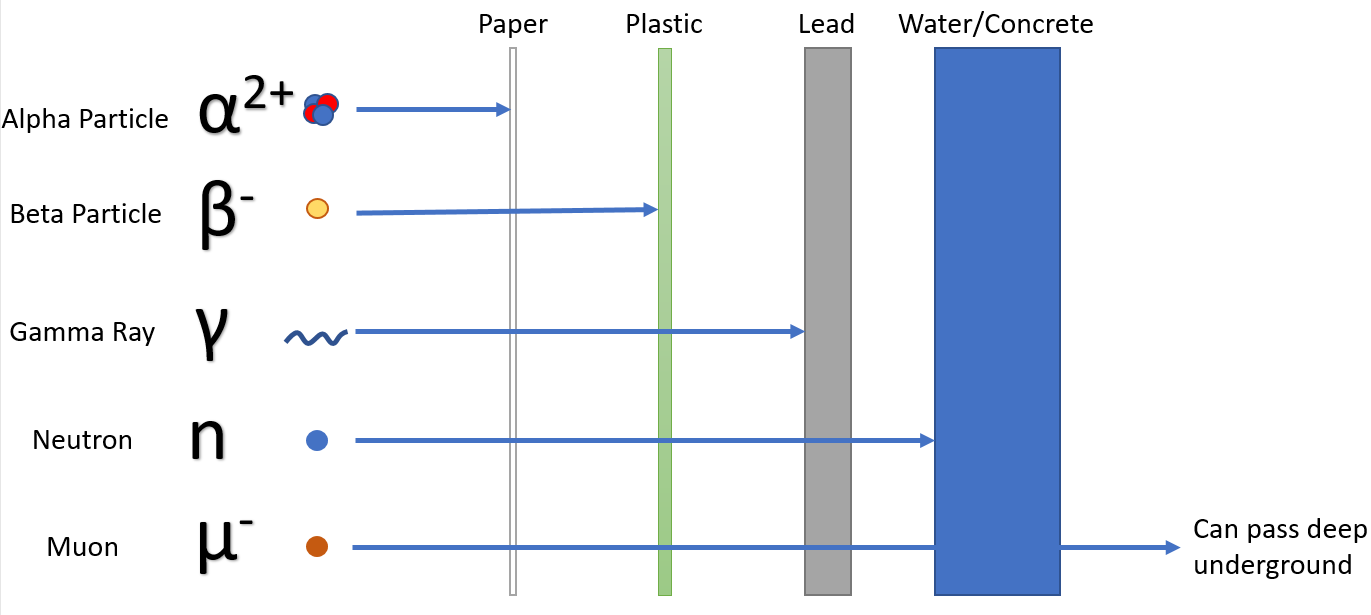
\includegraphics[width=\textwidth]{penetration}
\caption{Various penetration capabilities of several types of radiation}
\label{fig:penetration}
\end{figure}

\subsection{Alpha Particles}
While gamma rays are the dominant type of radiation that germanium detectors are designed to be sensitive to, the other types can still have an effect on measurements and energy spectra.
As shown in Figure \ref{fig:penetration}, alpha particles can be stopped by a thin sheet of paper.
However, they can still interact with the surface of a germanium detector and deposit their energy.
Most alphas would be blocked by the detector housing but some trace amounts of heavy radioactive elements can exist in the metal shielding.
These elements such as uranium 238 or thorium 232 can decay and eject an alpha particle inside the housing that might hit the detector.

As mentioned previously, alpha decay comes from unstable heavy nuclei that spontaneously emit energy in the form of a $^{4}$He nucleus.
The probablity of decay is determined by the barrier penetration mechanism and varies from element to element resulting in half lifes that rande from seconds to thousands of years.
The average kinetic energy of an alpha particle is around 4.6 MeV.
They typically interact through the coulomb force with the electrons in orbit around the absorber atom and can travel aproximately 2.5 cm in air before losing all of its energy.

\subsection{Beta Particles}
Beta particles are more likely than alpha particles to interact with a germanium detector but still unlikely due to them usualy being abosrbed by the detector housing.
Many nuclides decay via beta emission so it is still posible for decays to occur inside the shielding that could hit the detector, or the rare case that a beta would penetrate the housing.
Special detectors can also implement a beryllium window that would facilitate the passage of beta particles to the detector.
Betas lose energy much slower than alpha particles, through both coulomb and radiative processes, so their path through space can be winding and long.
Betas interact with orbital electrons due to them both being negatively charged.


\subsection{Neutrons}
Neutrons have the potential to interact with Ge detectors but due to them having no electric charge, they cannon interact via the coulomb force.
This means they can usually travel many centimeters through material without interacting at all.
For a neutron to deposit energy, it must interact with the nucleus of an atom.

Several classifications exist for neutrons based on the kinetic energy they have and determin which interaction is most likely.
The slowest neutrons are captured by nuclei.
This changes the atomic mass of the atom and can result in a decay which would create a gamma ray.
That gamma ray could then go on to interact with the detector and deposit its energy.
Faster neutrons can scatter off nucleus and deposit some energy.
If a neutron scatters elestically, it gives a nuclear recoil and changes direction.
If it scatters innelastically, it will give a nuclear recoil and can cause and excitation which would result in a gamma ray.
Finally, the fastes neutrons can undergo spallation.
Spallation is when an incoming neutron hits a nucleus and blows it appart and give off massive amounts of energy.

\subsection{Muons}
Muons are negatively charged particles, most of which come from cosmic rays, and are minimum ionizing. 
Muons can travel deep underground and can also create a huge deposition of energy in very short time.
Muons can also spallate.

\subsection{Gamma Rays}
As mentioned earlier, gamma rays are the primary radiation seen by germanium detectors.
Gamma rays have typical energy from 10's of KeV to 2.6 MeV being the highest energy to exist naturally.
Gamma rays can interact with a germanium detector in three ways: through the photoelectric effect, compton scattering, or pair production.
\begin{figure}[htpb]
\centering
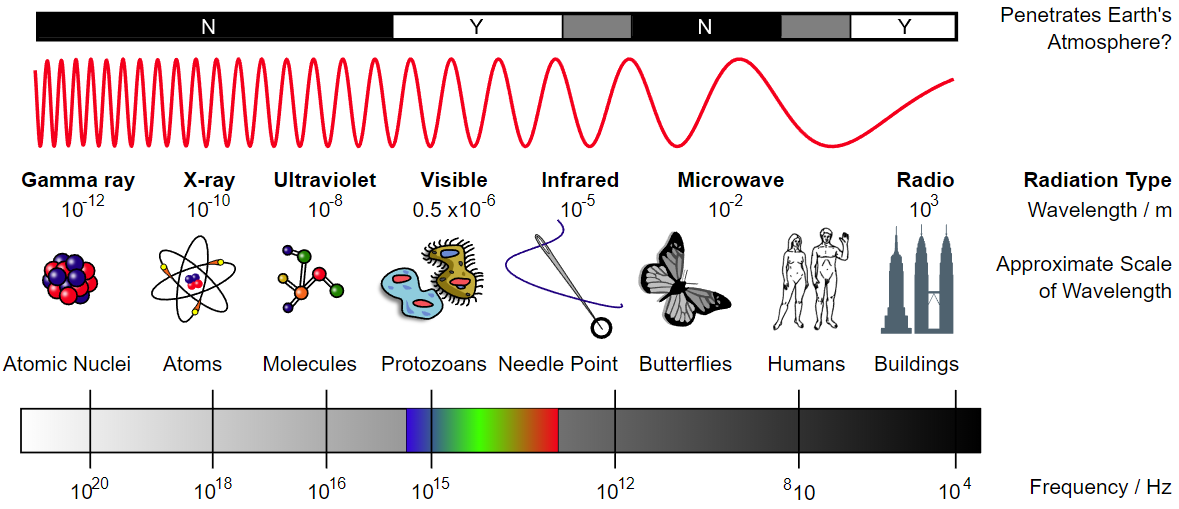
\includegraphics[width=\textwidth]{emspectra}
\caption{Spectrum of electromagnetic waves}
\label{fig:emspectra}
\end{figure}

The photoelectric efect got Einstein a nobel prize and is one of the most important interactions ligt can have with matter.
For the photoelectric effect to occur, an incoming electromagnetic wave must have energy higher than the energy binding the electron to the atom.
If it does, a gamma ray can hit and atom, be abosrbed, and eject an electron with kinetic energy proportional to the incoming gamma ray.
This electron will then wander around losing energy until it is ejected from the surface or stops.
The filling of the hole left by the ejected electron can also cause the emission of characteristic x-ray photons.

The second method, compton scattering, is the most common interaction of germanium detectors and gamma rays.
In compton scattering, the incoming gamma ray is deflected of an electron to which it transfers some amount of energy.
This recoil electron will then lose energy to the bulk.

The final interation is pair production.
Pair production can occur only if the gamma ray has an energy in excess of twice the rest mass of an electron.
The interaction takes place within the coulomb field of the nucleus and causes the gamma ray to disapear and be replaced by an electron positron pair.
The positron will go on to annihilate which results in the creation of two more gamma rays that could deposit some energy to the detector.

Protons, can behave like a neutron or muon, can interact with EM field or nucleus- might not be needed.

\section{Spectroscopy}

understand the spectrum based on energy, compton shoulder, peaks, overall shape, etc Knolls book Ch10.F.2
energy resolution-random process for creation of electrons and holes 2.9 eV (average energy required to create electron hole pair) can also be caused by electron noise. some trapping of electrons and holes.
energy calibration,

\section{semiconducter diode detector}
Read all of chapter 11, skip section VI, Channeling
Read chapter 12
